\documentclass[11pt]{article}

\usepackage[T1]{fontenc}
\usepackage[utf8]{inputenc}
\usepackage[spanish,provide=*]{babel}
\usepackage{mathpazo}
\usepackage[scaled=0.92]{helvet}
\usepackage{microtype}
\usepackage[margin=2.6cm]{geometry}
\usepackage{amsmath,amssymb,amsthm}
\usepackage{bm}
\usepackage{booktabs}
\usepackage{tabularx}
\usepackage{multirow}
\usepackage{graphicx}
\usepackage{caption}
\usepackage{subcaption}
\usepackage{enumitem}
\usepackage{xcolor}
\usepackage{tikz}
\usetikzlibrary{arrows.meta,positioning,calc,fit,backgrounds}
\usepackage{algorithm}
\usepackage{algpseudocode}
\usepackage[round,authoryear]{natbib}
\usepackage[colorlinks=true,linkcolor=blue!50!black,citecolor=blue!50!black,urlcolor=blue!50!black]{hyperref}

\captionsetup{font=small,labelfont=bf}
\urlstyle{same}
\setlist{itemsep=2pt,topsep=4pt}

\newtheorem{proposicion}{Proposición}
\theoremstyle{definition}
\newtheorem{definicion}{Definición}
\theoremstyle{remark}
\newtheorem{observacion}{Observación}

\floatname{algorithm}{Algoritmo}
\algrenewcommand\algorithmicrequire{\textbf{Entrada:}}
\algrenewcommand\algorithmicensure{\textbf{Salida:}}

\newcommand{\Pre}{\operatorname{Pre}}
\newcommand{\Rh}{\hat R}
\newcommand{\Sh}{\hat S}
\newcommand{\Lh}{\hat L}
\newcommand{\Pih}{\hat\Pi}
\newcommand{\rstar}{r^{\ast}}
\newcommand{\Slisto}{S_{\mathrm{listo}}}
\newcommand{\Smin}{S_{\min}}

\definecolor{azul}{HTML}{2A78D6}
\definecolor{naranja}{HTML}{EB6834}
\definecolor{gris}{HTML}{52514E}

\title{\textbf{Repetición espaciada sobre grafos de habilidades procedimentales}\\[4pt]
\large Un modelo de memoria con crédito fraccional, asignación bayesiana de culpa,\\
admisión con control de carga y planificación por cobertura submodular}
\author{Gustavo S. de la Rosa\\[2pt]\small Proyecto de maestría --- borrador para revisión con el asesor}
\date{Octubre de 2026}

\begin{document}
\maketitle

\begin{abstract}
\noindent Los sistemas de repetición espaciada se han diseñado para memorizar hechos aislados: cada tarjeta ejercita un solo elemento de conocimiento. En física y matemáticas de preparatoria, en cambio, resolver un problema exige ejecutar varios procedimientos que dependen unos de otros. Proponemos un modelo para planificar la práctica de habilidades procedimentales que combina tres piezas: (i) un grafo de prerrequisitos con una matriz $Q$ fraccional, según la cual un problema ejercita por completo su tema y parcialmente sus prerrequisitos; (ii) el modelo de olvido exponencial $R(t)=e^{-\Delta t/S}$ con la dinámica de saltos de \citet{tabibian2019}, extendida a problemas con varias habilidades mediante un modelo de observación conjuntivo con descuido y adivinanza y una asignación bayesiana de culpa tras los fallos; y (iii) un planificador por sesión que admite temas nuevos sólo si sus prerrequisitos están consolidados y la carga de mantenimiento cabe en el presupuesto, y que elige los problemas maximizando una función de cobertura submodular, con garantía de aproximación $1-1/e$ para el algoritmo voraz. Los parámetros se estiman por máxima verosimilitud con datos de un piloto. Evaluamos el modelo con un simulador Monte Carlo cuyo alumno ``verdadero'' está deliberadamente mal especificado respecto al modelo (olvido de ley de potencia, ganancia tipo FSRS, recuperación oculta por componente), sobre el grafo de mecánica de preparatoria a nivel de 15 unidades y de 168 subtemas. A nivel de unidades, con presupuesto holgado, el modelo no supera a un Anki SM-2 bien configurado. A nivel de subtemas, donde el presupuesto es escaso, supera a Anki en $+0.090$ y $+0.047$ de probabilidad media de resolver un problema nuevo 30 días después del curso. La ventaja proviene sobre todo de una mayor cobertura y no de una mejor retención por tema, y desaparece si el grafo contiene dependencias falsas. Discutimos las limitaciones y proponemos un diseño experimental para el aula.
\end{abstract}

\tableofcontents
\bigskip

%=====================================================================
\section{Introducción}
%=====================================================================

La repetición espaciada es una de las estrategias de aprendizaje con mejor respaldo empírico \citep{cepeda2006,cepeda2008}. Sus implementaciones más difundidas, de SM-2 \citep{wozniak1990} a FSRS \citep{ye2022}, y los enfoques de control óptimo como MEMORIZE \citep{tabibian2019}, comparten un supuesto: cada elemento a repasar es independiente y ejercita una sola pieza de conocimiento. \citet{choffin2021} lo resumen así: ``hasta donde sabemos, todos los algoritmos de espaciado adaptativo están diseñados para aprender piezas simples de conocimiento, ítems que involucran un solo componente''.

Resolver problemas de física rompe ese supuesto de tres maneras:
\begin{enumerate}[label=(\alph*)]
\item un problema de tiro parabólico exige recuperar a la vez la descomposición de vectores, las ecuaciones del movimiento acelerado y la independencia de los movimientos, así que cada intento aporta evidencia sobre varias habilidades;
\item un fallo no dice cuál de ellas falló;
\item existe un orden natural de aprendizaje: introducir un tema antes de que sus bases estén firmes desperdicia práctica, e introducir demasiados temas a la vez satura la cola de repasos \citep{reddy2016}.
\end{enumerate}

Este trabajo propone un modelo que integra esas tres consideraciones sobre la ecuación de olvido $R(t)=e^{-n\,\Delta t}$ de \citet{tabibian2019}. La idea central es repartir las responsabilidades así: \emph{el grafo decide qué está listo para aprender y por dónde fluye la práctica; el modelo de memoria decide qué se está desvaneciendo; y el planificador elige los problemas que cubren mejor lo que se desvanece.}

\paragraph{Contribuciones.}
\begin{enumerate}
\item \textbf{Modelo de observación multihabilidad} (\S\ref{sec:modelo}). Extiende la dinámica de saltos de Tabibian a problemas con varias habilidades mediante pesos fraccionarios $w_{jk}$, un modelo conjuntivo con descuido y adivinanza, y una regla de culpa basada en la probabilidad posterior de que cada componente haya fallado.
\item \textbf{Admisión con invariante de carga} (\S\ref{sec:admision}). Convierte la observación de saturación de \citet{reddy2016} en una condición explícita: no se admite un tema nuevo si la carga esperada de mantenimiento excede una fracción del presupuesto.
\item \textbf{Planificador por cobertura submodular} (\S\ref{sec:planificador}), con garantía de aproximación $1-1/e$ para el algoritmo voraz (Proposición~\ref{prop:submod}).
\item \textbf{Protocolo de evaluación por simulación con verdad mal especificada} (\S\ref{sec:simulador}). Incluye estimación de parámetros por máxima verosimilitud a partir de un piloto, igual que se haría con datos reales.
\item \textbf{Evidencia de simulación} sobre el grafo de mecánica de preparatoria (\S\ref{sec:resultados}): la ventaja del modelo depende de la granularidad del grafo, del presupuesto y de la fidelidad de las dependencias.
\end{enumerate}

%=====================================================================
\section{Trabajo relacionado}
\label{sec:relacionado}
%=====================================================================

\paragraph{Planificación de repasos.}
\citet{tabibian2019} modelan los repasos como un proceso puntual marcado y derivan la intensidad óptima $u^\ast(t)=q^{-1/2}(1-m(t))$ bajo una pérdida cuadrática. Su resultado supone ítems independientes, un costo suave sobre la intensidad y tiempos muestreados de un proceso de Poisson. Los propios autores dejan como trabajo futuro el caso de ítems dependientes. \citet{upadhyay2021} adaptan el enfoque a la selección de ítems dentro de sesiones elegidas por el usuario y lo validan con un experimento aleatorizado a gran escala. \citet{reddy2016} modelan el sistema Leitner como una red de colas y muestran una transición de fase: por encima de cierta tasa de llegada de ítems nuevos, el sistema se satura. FSRS \citep{ye2022,su2023}, hoy integrado en Anki, usa un modelo de dificultad, estabilidad y recuperabilidad con un efecto de espaciamiento explícito. \citet{hunziker2019} dan garantías para enseñar varios conceptos a un aprendiz que olvida, mediante funciones submodulares.

\paragraph{Ítems con varias habilidades.}
DAS3H \citep{choffin2019} extiende los modelos aditivos de factores con ventanas temporales de olvido por habilidad. \citet{choffin2021} extienden heurísticas de espaciado a ítems con varias habilidades mediante selección voraz de subconjuntos; es el antecedente más cercano a nuestro planificador. Math Academy describe un esquema propietario (\emph{Fractional Implicit Repetition}) en el que el crédito por resolver temas avanzados ``fluye'' fraccionalmente hacia sus componentes \citep{skycak2023}. Hasta donde sabemos, no tiene un modelo publicado ni una evaluación controlada.

\paragraph{Modelos de estudiante y diagnóstico.}
El rastreo bayesiano del conocimiento \citep{corbett1994} introdujo los parámetros de descuido y adivinanza que usamos. Los modelos de diagnóstico cognitivo con matriz $Q$ \citep{tatsuoka1983}, como DINA \citep{junker2001} y G-DINA \citep{delatorre2011}, formalizan el modelo conjuntivo. PFA \citep{pavlik2009} y AFM \citep{cen2006} son las alternativas aditivas. El marco KLI \citep{koedinger2012} define los componentes de conocimiento y advierte que su granularidad es una cuestión empírica.

\paragraph{Admisión por prerrequisitos.}
La teoría de espacios de conocimiento \citep{doignon1985} define el \emph{outer fringe}: los ítems que un estudiante está listo para aprender. Nuestra regla de admisión es un \emph{outer fringe} en el que ``saber'' se sustituye por ``estabilidad suficiente''.

\paragraph{Evidencia sobre espaciamiento en procedimientos.}
El espaciamiento y el intercalado mejoran el aprendizaje de matemáticas \citep{rohrer2007,rohrer2015}, aunque la evidencia para procedimientos es menos robusta que para hechos \citep{barzagar2019}. La hipótesis del esfuerzo de recuperación \citep{pyc2009} sostiene que las recuperaciones difíciles pero exitosas fortalecen más la memoria. Las habilidades cognitivas decaen con el desuso \citep{arthur1998}, pero la forma funcional de ese decaimiento no está establecida.

%=====================================================================
\section{Modelo}
\label{sec:modelo}
%=====================================================================

\subsection{Grafo de habilidades y matriz \texorpdfstring{$Q$}{Q} fraccional}

Sea $G=(V,E)$ un grafo dirigido acíclico de $K$ habilidades, donde $(p,k)\in E$ significa que $p$ es prerrequisito de $k$. Denotamos $\Pre(k)=\{p:(p,k)\in E\}$. Cada habilidad $j$ tiene asociado un tipo de problema (en la práctica, un banco de problemas) que ejercita $j$ y, parcialmente, sus prerrequisitos directos:
\begin{equation}
w_{jk}=\begin{cases}1 & k=j,\\ w_{\mathrm{pre}} & k\in\Pre(j),\\ 0 & \text{en otro caso,}\end{cases}
\qquad Q(j)=\{j\}\cup\Pre(j).
\label{eq:pesos}
\end{equation}
La matriz $W=(w_{jk})$ es una matriz $Q$ con entradas fraccionarias. En este trabajo usamos $w_{\mathrm{pre}}=0.5$; con datos reales, los $w_{jk}$ pueden estimarse (\S\ref{sec:futuro}). La Figura~\ref{fig:grafo-ejemplo} muestra un ejemplo.

\begin{figure}[t]
\centering
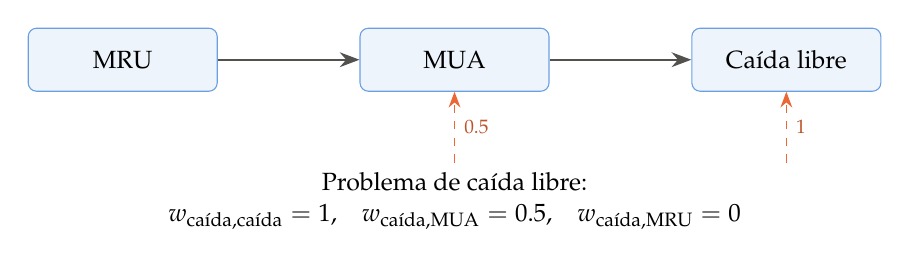
\begin{tikzpicture}[
  nodo/.style={draw, rounded corners=3pt, minimum height=8mm, minimum width=24mm, font=\small, fill=azul!8, draw=azul!70},
  pre/.style={-{Stealth[length=2.5mm]}, thick, gris},
  peso/.style={font=\scriptsize, text=naranja!80!black}
]
\node[nodo] (mru) {MRU};
\node[nodo, right=18mm of mru] (mua) {MUA};
\node[nodo, right=18mm of mua] (cai) {Caída libre};
\draw[pre] (mru) -- (mua);
\draw[pre] (mua) -- (cai);
\node[font=\small, below=9mm of mua, align=center] (prob) {Problema de caída libre:\\
$w_{\text{caída},\text{caída}}=1$,\quad $w_{\text{caída},\text{MUA}}=0.5$,\quad $w_{\text{caída},\text{MRU}}=0$};
\draw[-{Stealth[length=2mm]}, naranja, dashed] (prob.north -| cai) -- node[peso, right]{1} (cai.south);
\draw[-{Stealth[length=2mm]}, naranja, dashed] (prob.north -| mua) -- node[peso, right]{0.5} (mua.south);
\end{tikzpicture}
\caption{Grafo mínimo y la fila de la matriz $Q$ fraccional de un problema de caída libre. Las flechas grises son prerrequisitos; las punteadas indican cuánto ejercita el problema cada habilidad.}
\label{fig:grafo-ejemplo}
\end{figure}

\subsection{Estado y modelo de memoria}

Para cada habilidad introducida, el planificador mantiene una estabilidad $\Sh_k>0$ (en días) y un instante efectivo del último repaso $\Lh_k$. La probabilidad de recuerdo creída es el modelo exponencial de \citet{tabibian2019}:
\begin{equation}
\Rh_k(t)=\exp\!\left(-\frac{t-\Lh_k}{\Sh_k}\right)=e^{-\hat n_k\,\Delta t},\qquad \hat n_k=1/\Sh_k,
\label{eq:memoria}
\end{equation}
y $\Rh_k\equiv 0$ si $k$ no se ha introducido. Al introducir $k$ se fija $\Sh_k=\Sh_0$ y $\Lh_k=t$.

\subsection{Modelo de observación}

Un intento del problema $j$ produce un resultado binario $y\in\{0,1\}$. Suponemos un modelo \emph{conjuntivo}: el alumno resuelve el problema si recupera todos sus componentes, salvo un descuido con probabilidad $s$, y si falla alguno puede acertar por adivinanza con probabilidad $g$. El exponente $w_{jk}$ hace que un componente parcial sea más fácil de ``pasar'':
\begin{equation}
\Pih_j(t)=\prod_{k\in Q(j)}\Rh_k(t)^{\,w_{jk}},\qquad
\hat P_j(t)=\Pr(y=1)=(1-s)\,\Pih_j(t)+g\,\bigl(1-\Pih_j(t)\bigr).
\label{eq:observacion}
\end{equation}
Usamos $s=0.05$ (error aritmético o de transcripción aun sabiendo) y $g=0.02$ (los problemas son abiertos, así que acertar sin saber es raro).

\subsection{Actualización tras un intento}

Cada habilidad se actualiza \textbf{a lo sumo una vez por sesión}, como en el tratamiento de los datos de Duolingo de \citet{tabibian2019}. Los intentos repetidos el mismo día ocurren con $\Rh\approx1$ y no aportan evidencia sobre la memoria de largo plazo. Las habilidades introducidas en la sesión tampoco se actualizan.

\paragraph{Acierto.} Todos los componentes se recuperaron, así que cada uno recibe crédito proporcional a su peso:
\begin{equation}
\Sh_k\leftarrow \Sh_k\bigl[1+w_{jk}\,G\,(1-\Rh_k)\bigr],\qquad k\in Q(j).
\label{eq:acierto}
\end{equation}
La ganancia es nula si $\Rh_k=1$ y crece cuando la recuperación era difícil. Así se modela el efecto de espaciamiento y la práctica masiva no puede ``dominar'' un tema.

\paragraph{Salto del recuerdo.} Tras cualquier intento el alumno ve la solución, y el recuerdo salta según la ecuación de \citet{tabibian2019}, $dm=(1-m)\,dN$, ponderada por $w$:
\begin{equation}
\Rh_k^{+}=\Rh_k+w_{jk}(1-\Rh_k),\qquad \Lh_k\leftarrow t+\Sh_k^{+}\ln\Rh_k^{+}.
\label{eq:salto}
\end{equation}
La segunda expresión elige el $\Lh_k$ que reproduce $\Rh_k^+$ con la nueva estabilidad, de modo que el olvido continúe desde ahí.

\paragraph{Fallo y asignación de culpa.} El sistema sólo observa que el problema falló, no qué componente falló. La culpa de cada componente es la probabilidad posterior de que no se haya recuperado:
\begin{equation}
b_k=\min\!\left(1,\ \frac{1-\Rh_k^{\,w_{jk}}}{1-\Pih_j}\right),\qquad
\Sh_k\leftarrow\max\bigl(\Smin,\ \Sh_k(1-\lambda\,b_k)\bigr),
\label{eq:culpa}
\end{equation}
seguida del salto~\eqref{eq:salto}. Las $b_k$ son probabilidades marginales, así que pueden sumar más de uno: es posible que fallen varias habilidades a la vez. La expresión~\eqref{eq:culpa} ignora $s$ y $g$; la versión completa es
\begin{equation}
b_k^{\mathrm{completa}}=\frac{(1-\Rh_k^{\,w_{jk}})(1-g)}{(1-\Pih_j)(1-g)+\Pih_j\,s},
\label{eq:culpa-completa}
\end{equation}
que reduce mucho la culpa cuando $\Pih_j\approx1$: un fallo así es más probablemente un descuido que un olvido. Su implementación queda como trabajo futuro (\S\ref{sec:futuro}).

\paragraph{Ejemplo.} Supongamos $\Rh_{\text{caída}}=0.643$ y $\Rh_{\text{MUA}}=0.793$. Entonces $\Pih=0.643\cdot0.793^{0.5}=0.573$. Si el problema de caída libre falla, $b_{\text{caída}}=0.357/0.427=0.84$ y $b_{\text{MUA}}=0.110/0.427=0.26$: el sistema atribuye el fallo casi por completo a caída libre (Apéndice~\ref{app:traza}).

\subsection{Admisión con control de carga}
\label{sec:admision}

Con $\rstar$ como retención objetivo, la habilidad $k$ vuelve a vencer aproximadamente cada $\Sh_k\ln(1/\rstar)$ días. La \emph{carga} esperada de mantenimiento, en repasos por sesión (5 sesiones por semana), es
\begin{equation}
\mathcal L=\sum_{k\ \text{introducida}}\min\!\left(1,\ \frac{7/5}{\Sh_k\ln(1/\rstar)}\right).
\label{eq:carga}
\end{equation}

\begin{definicion}[Admisibilidad]
Una habilidad $k$ no introducida es \emph{admisible} en el instante $t$ si
\begin{equation}
\underbrace{\forall p\in\Pre(k):\ \Sh_p\ge\Slisto\ \wedge\ \Rh_p(t)\ge\rstar}_{\text{está lista}}
\qquad\text{y}\qquad
\underbrace{\mathcal L+m+1\le\rho\,U}_{\text{cabe}},
\label{eq:admision}
\end{equation}
donde $U$ es el número de problemas por sesión, $\rho\in(0,1)$ la fracción máxima que puede ocupar el mantenimiento y $m$ el número de temas ya admitidos en la sesión. Entre las admisibles se elige la primera en el orden del libro. Se admiten hasta $m_{\max}$ temas por sesión, y cada introducción cuesta $n_{\mathrm{intro}}$ lugares (ejemplo resuelto y práctica inicial).
\end{definicion}

La primera condición es el \emph{outer fringe} de \citet{doignon1985} con ``estable'' en lugar de ``sabido''. La segunda convierte la condición de estabilidad de \citet{reddy2016} en un invariante: si el modelo de memoria es correcto, la carga esperada nunca excede $\rho U$.

\subsection{Planificador de la sesión}
\label{sec:planificador}

Sean $D=\{k:\Rh_k(t)<\rstar\}$ las habilidades vencidas, con prioridad $\pi_k=1-\Rh_k(t)$. Esta prioridad tiene la forma de la intensidad óptima de Tabibian, $u^\ast\propto 1-m$, convertida en una decisión diaria. Un problema $j$ es \emph{factible} si todos sus otros componentes cumplen $\Rh_c\ge r_{\min}$; así se evitan problemas cuyos fallos no diagnosticarían nada. Para un conjunto $A$ de problemas factibles definimos
\begin{equation}
V(A)=\sum_{k\in D}\pi_k\Bigl[1-\prod_{j\in A}(1-w_{jk})\Bigr].
\label{eq:cobertura}
\end{equation}
El corchete es la fracción de la habilidad $k$ cubierta por $A$: un problema principal la cubre entera, y dos problemas que la usan como prerrequisito cubren $1-0.5^2=75\%$.

\begin{proposicion}
\label{prop:submod}
$V$ es no negativa, monótona y submodular. Por lo tanto, el algoritmo voraz que agrega en cada paso el problema de mayor ganancia marginal
\begin{equation}
\Delta(j\mid A)=\sum_{k\in D}\pi_k\,\eta_k(A)\,w_{jk},\qquad \eta_k(A)=\prod_{j'\in A}(1-w_{j'k}),
\label{eq:ganancia}
\end{equation}
hasta $U$ elementos, obtiene $V(A_{\mathrm{voraz}})\ge(1-1/e)\max_{|A|\le U}V(A)$.
\end{proposicion}
\begin{proof}[Esbozo de prueba]
Para cada $k$, $f_k(A)=1-\prod_{j\in A}(1-w_{jk})$ es la probabilidad de que ocurra al menos uno de varios eventos independientes con probabilidades $w_{jk}$, es decir, una función de cobertura probabilística. Es monótona, y su ganancia marginal $w_{jk}\prod_{j'\in A}(1-w_{j'k})$ no crece al agrandar $A$, lo que la hace submodular. Una combinación no negativa de funciones submodulares monótonas es submodular monótona, y el resultado se sigue de \citet{nemhauser1978}.
\end{proof}

\begin{observacion}
La garantía se refiere a $V$, que es un sustituto de lo que realmente interesa: la retención futura. No es una garantía sobre el aprendizaje. Además, la implementación se detiene si la ganancia marginal es menor que $\varepsilon$, lo que introduce una pérdida aditiva de a lo sumo $\varepsilon U$.
\end{observacion}

El Algoritmo~\ref{alg:sesion} resume una sesión. Los lugares sobrantes se llenan con el problema factible de menor $\Rh$ que aún no venció.

\begin{algorithm}[t]
\caption{Planificación de una sesión ($\eta_k$ es la fracción de $k$ aún sin cubrir)}
\label{alg:sesion}
\small
\begin{algorithmic}[1]
\Require estado $(\Sh_k,\Lh_k)$, presupuesto $U$, parámetros $\rstar,r_{\min},\Slisto,\rho,m_{\max},n_{\mathrm{intro}}$
\State calcular $\Rh_k(t)$ con~\eqref{eq:memoria}; $D\gets\{k:\Rh_k<\rstar\}$; $\pi_k\gets1-\Rh_k$; $\eta_k\gets1$
\State $A\gets\emptyset$
\While{$|A|<U$ y existe $j$ factible $\notin A$ con $\Delta(j\mid A)>\varepsilon$} \Comment{cobertura voraz}
  \State $j^\ast\gets\arg\max_j\Delta(j\mid A)$; \ $A\gets A\cup\{j^\ast\}$; \ $\eta_k\gets\eta_k(1-w_{j^\ast k})$
\EndWhile
\State $N\gets\emptyset$
\While{$|N|<m_{\max}$ y quedan $\ge n_{\mathrm{intro}}$ lugares y hay $k$ admisible según~\eqref{eq:admision}} \Comment{admisión}
  \State $N\gets N\cup\{k\}$
\EndWhile
\State llenar los lugares restantes con problemas factibles de menor $\Rh$
\State \textbf{para cada} intento observado: actualizar con~\eqref{eq:acierto}--\eqref{eq:culpa}, una vez por habilidad
\end{algorithmic}
\end{algorithm}

\subsection{Estimación de parámetros}

Los parámetros $\bm\phi=(\Sh_0,G,\lambda)$ se estiman por máxima verosimilitud a partir de los registros de un piloto. Para cada alumno $i$ se ``reproduce'' su historia como un filtro: se predice $\hat P_{in}$ con~\eqref{eq:observacion}, se observa $y_{in}$ y se actualiza con~\eqref{eq:acierto}--\eqref{eq:culpa}. La log-verosimilitud negativa es
\begin{equation}
\mathrm{NLL}(\bm\phi)=-\sum_i\sum_n\Bigl[y_{in}\ln\hat P_{in}(\bm\phi)+(1-y_{in})\ln\bigl(1-\hat P_{in}(\bm\phi)\bigr)\Bigr],
\label{eq:nll}
\end{equation}
y se minimiza con Nelder--Mead sobre $(\ln\Sh_0,\ln G,\operatorname{logit}\lambda)$, lo que evita restricciones. Los parámetros $s$, $g$ y $\Smin$ se fijan.

%=====================================================================
\section{Simulador}
\label{sec:simulador}
%=====================================================================

Evaluar el planificador con el mismo modelo con el que se generan los datos garantiza el éxito por construcción. Por eso el simulador separa la \emph{verdad} (cómo aprende y olvida el alumno simulado, que el planificador nunca ve) del \emph{modelo} (\S\ref{sec:modelo}), y especifica mal el segundo respecto a la primera a propósito (Tabla~\ref{tab:verdad-modelo}).

\begin{table}[t]
\centering\small
\caption{Diferencias deliberadas entre la verdad simulada y el modelo del planificador.}
\label{tab:verdad-modelo}
\begin{tabularx}{\textwidth}{lXX}
\toprule
& Verdad (alumno simulado) & Modelo (planificador) \\
\midrule
Olvido & ley de potencia, $R=(1+F\Delta t/S)^{C}$ & exponencial, $\Rh=e^{-\Delta t/\Sh}$ \\
Ganancia & $\gamma S^{-b}\,(e^{c(1-R)}-1)$, tipo FSRS & $G(1-\Rh)$ \\
Fallo & lapso en los componentes que de verdad no se recuperaron & culpa repartida con~\eqref{eq:culpa} \\
Bases débiles & según el escenario & sólo la compuerta de admisión \\
Heterogeneidad & $\theta_i\sim N(0,0.35^2)$ & ninguna \\
\bottomrule
\end{tabularx}
\end{table}

\subsection{Alumno simulado}

Cada alumno tiene una habilidad latente $\theta_i\sim N(0,\sigma_\theta^2)$. Sea $\tilde d_k=c_d\,d_k$ la profundidad escalada de la habilidad $k$ en el grafo, con $c_d=1$ para el grafo de unidades y $c_d=6/\max_k d_k$ para los grafos de subtemas, de modo que la dificultad máxima sea comparable. Con esto se definen
\begin{gather}
S^{0}_{ik}=S_0\,e^{\theta_i-\delta\tilde d_k},\qquad \gamma_{ik}=e^{a+0.5\,\theta_i-0.1\,\tilde d_k},\label{eq:v-alumno}\\
R_k(t)=\Bigl(1+F\,\tfrac{t-L_k}{S_k}\Bigr)^{C},\qquad F=19/81,\ C=-0.5,\label{eq:v-olvido}
\end{gather}
de modo que $R(S)=0.9$: $S$ es el número de días en que el recuerdo cae a 90\%.

\paragraph{Introducción.} El tema arranca con una estabilidad que depende de la disponibilidad de sus prerrequisitos:
\begin{equation}
S_k=\max\Bigl(\Smin,\ S^{0}_{ik}\prod_{p\in\Pre(k)}r_p^{\,w_{\mathrm{pre}}}\Bigr),\qquad
r_p=\begin{cases}R_p(t) & \text{escenario A},\\ R_p(t)\bigl(1-e^{-S_p/\kappa}\bigr) & \text{escenario B}.\end{cases}
\label{eq:v-intro}
\end{equation}

\paragraph{Intento.} Para cada componente se sortea su recuperación, $\mathrm{ok}_k\sim\mathrm{Bernoulli}(R_k^{\,w_{jk}})$. El resultado observado es $y\sim\mathrm{Bernoulli}(1-s)$ si todos se recuperaron y $y\sim\mathrm{Bernoulli}(g)$ en otro caso. La memoria cambia según lo que \emph{realmente} se recuperó, no según $y$:
\begin{align}
\text{recuperó:}\quad & S_k\leftarrow S_k\bigl[1+w_{jk}\,c_k\,\gamma_{ik}\,S_k^{-b}\bigl(e^{c(1-R_k)}-1\bigr)\bigr],\label{eq:v-exito}\\
\text{no recuperó:}\quad & S_k\leftarrow\max\bigl(\Smin,\ S_k(1-\ell\,w_{jk})\bigr),\label{eq:v-lapso}\\
\text{en ambos casos:}\quad & L_k\leftarrow t-(1-w_{jk})(t-L_k).\label{eq:v-reloj}
\end{align}
En el escenario B, $c_k=\prod_{p\in\Pre(k)}(1-e^{-S_p/\kappa})^{w_{\mathrm{pre}}}$: mientras los prerrequisitos sigan frágiles, cada repaso de $k$ consolida menos. En el escenario A, $c_k=1$. La Tabla~\ref{tab:param-verdad} lista los valores.

\begin{table}[t]
\centering\small
\caption{Parámetros de la verdad simulada.}
\label{tab:param-verdad}
\begin{tabular}{lll}
\toprule
Parámetro & Valor & Interpretación \\
\midrule
$\sigma_\theta$ & 0.35 & heterogeneidad entre alumnos (escala logarítmica) \\
$S_0$ & 0.6 días & estabilidad de un tema recién visto \\
$\delta$ & 0.15 & penalización por profundidad en el grafo \\
$a$ & $\ln 4$ & escala de la ganancia por repaso \\
$b$ & 0.15 & rendimientos decrecientes en $S$ \\
$c$ & 2 & fuerza del efecto de espaciamiento \\
$\ell$ & 0.6 & fracción de estabilidad perdida en un lapso \\
$\kappa$ & 4 días & escala de consolidación de prerrequisitos \\
$s,\ g$ & 0.05, 0.02 & descuido y adivinanza \\
$\Smin$ & 0.2 días & piso de estabilidad \\
\bottomrule
\end{tabular}
\end{table}

\subsection{Políticas comparadas}

\begin{itemize}
\item \textbf{Propuesto}, con $\rstar=0.7$, $r_{\min}=0.6$, $\Slisto=7$ (en la escala del modelo), $\rho=0.8$ y $\varepsilon=10^{-3}$. También se evalúa con $\rstar=0.9$.
\item \textbf{Ablaciones}: sin crédito implícito ($w_{\mathrm{pre}}=0$ en el modelo), sin culpa bayesiana ($b_k=1$), sin control de carga y sin compuerta de prerrequisitos.
\item \textbf{Anki SM-2}: una tarjeta por tema, introducidas en orden del libro (hasta $m_{\max}$ por día), con intervalos $1, 6, I\cdot E$ y facilidad inicial $E=2.5$.
\item \textbf{Libro bloqueado}: un tema (o $\lceil K/60\rceil$ temas) por sesión en orden del libro, sin repaso.
\item \textbf{Libro con repaso acumulativo}: igual que el anterior, pero 2 de los $U$ problemas son de temas anteriores al azar.
\end{itemize}

\subsection{Diseño de la simulación}

El curso dura 12 semanas con 5 sesiones por semana (60 sesiones). La métrica principal es la probabilidad media, sobre \emph{todas} las habilidades del grafo, de que el alumno resuelva un problema nuevo de cada una, evaluada 30 días después de la última sesión y sin práctica intermedia:
\begin{equation}
\text{Examen}_i=\frac1K\sum_{k=1}^K P_{ik}(T_{\mathrm{test}}).
\label{eq:examen}
\end{equation}
Un tema no introducido vale $g=0.02$, así que la métrica premia tanto la retención como la cobertura. Cada política se aplica a los mismos $N=300$ alumnos, y las diferencias se reportan pareadas por alumno con IC del 95\%. Los parámetros $(\Sh_0,G,\lambda)$ se estiman por escenario con un piloto de 100 alumnos distintos, en el que los temas se introducen en orden del libro y se repasan al azar.

\paragraph{Grafos.}
\begin{itemize}
\item \textbf{Unidades}: el grafo de mecánica de preparatoria con 15 unidades y 26 aristas, de magnitudes y unidades a movimiento de rotación, con profundidad máxima 8. Configuración: $U=6$, $n_{\mathrm{intro}}=3$, $m_{\max}=1$.
\item \textbf{Subtemas}: los 168 subtemas de esas unidades, con 279 dependencias anotadas manualmente a nivel de subtema (profundidad máxima 20). Configuración: $U=10$, $n_{\mathrm{intro}}=2$, $m_{\max}=3$.
\item \textbf{Subtemas lineales}: control estructural. Cada unidad es una cadena lineal de sus subtemas, y cada arista entre unidades conecta el último subtema de la unidad origen con el primero de la destino (profundidad máxima 103).
\end{itemize}

%=====================================================================
\section{Resultados}
\label{sec:resultados}
%=====================================================================

\subsection{Grafo de unidades: presupuesto holgado}

Con 15 unidades y 60 sesiones hay cuatro sesiones por tema, y todas las políticas introducen las 15 unidades. La Tabla~\ref{tab:unidades} muestra que cualquier política con repaso espaciado supera al libro bloqueado por $0.28$--$0.29$, pero el sistema propuesto no supera a Anki SM-2 (diferencias de $+0.006$ y $+0.008$ a favor de Anki). La compuerta de prerrequisitos le cuesta $0.009$--$0.011$, porque retrasa la introducción de temas en un grafo profundo. La ventaja sobre Anki sólo aparece con presupuesto escaso ($U=4$): $0.731$ frente a $0.714$ en A y $0.695$ frente a $0.681$ en B.

\begin{table}[t]
\centering\small
\caption{Grafo de 15 unidades ($U=6$). Examen diferido (media $\pm$ IC95\%) y diferencia pareada respecto al propuesto. Estimaciones del piloto: $\Sh_0=5.23$, $G=6.07$, $\lambda=0.09$ (A); $\Sh_0=4.71$, $G=4.26$, $\lambda=0.11$ (B).}
\label{tab:unidades}
\begin{tabular}{lcccc}
\toprule
& \multicolumn{2}{c}{A: bases débiles, efecto leve} & \multicolumn{2}{c}{B: efecto persistente} \\
\cmidrule(lr){2-3}\cmidrule(lr){4-5}
Política & Examen & $\Delta$ & Examen & $\Delta$ \\
\midrule
Propuesto ($\rstar=0.7$) & $0.743\pm0.004$ & --- & $0.714\pm0.005$ & --- \\
Propuesto ($\rstar=0.9$) & $0.728\pm0.004$ & $-0.015$ & $0.677\pm0.006$ & $-0.038$ \\
\quad sin crédito implícito & $0.742\pm0.004$ & $-0.001$ & $0.713\pm0.005$ & $-0.001$ \\
\quad sin culpa bayesiana & $0.741\pm0.004$ & $-0.002$ & $0.711\pm0.005$ & $-0.003$ \\
\quad sin control de carga & $0.741\pm0.004$ & $-0.002$ & $0.714\pm0.005$ & $+0.000$ \\
\quad sin compuerta & $0.753\pm0.004$ & $+0.011$ & $0.723\pm0.005$ & $+0.009$ \\
Anki SM-2 & $0.749\pm0.004$ & $+0.006$ & $0.722\pm0.005$ & $+0.008$ \\
Libro + repaso acumulativo & $0.628\pm0.004$ & $-0.115$ & $0.605\pm0.005$ & $-0.110$ \\
Libro bloqueado & $0.463\pm0.005$ & $-0.280$ & $0.427\pm0.006$ & $-0.287$ \\
\bottomrule
\end{tabular}
\end{table}

\subsection{Grafo de subtemas: presupuesto escaso}

Con 168 subtemas ninguna política adaptativa alcanza a introducirlos todos en 60 sesiones, y la situación cambia (Tabla~\ref{tab:subtemas}, Figura~\ref{fig:subtemas}):

\begin{itemize}
\item \textbf{El propuesto supera a Anki} por $+0.090$ (A) y $+0.047$ (B), y la ventaja se mantiene con $U\in\{6,10,14\}$ (Figura~\ref{fig:presupuesto}).
\item \textbf{El mecanismo es la cobertura}: Anki acumula repasos vencidos y deja de introducir temas (71 frente a 106 en A; 63 frente a 79 en B; Figura~\ref{fig:trayectorias}).
\item \textbf{El crédito implícito} aporta $+0.014$ en A, porque un problema avanzado repasa de paso varios subtemas cuando los lugares escasean.
\item \textbf{La compuerta} aporta $+0.015$ en B, donde aprender sobre bases frágiles hace daño persistente.
\item \textbf{La culpa bayesiana} aporta poco: $+0.002$ a $+0.004$.
\end{itemize}

\begin{table}[t]
\centering\small
\caption{Grafo de 168 subtemas ($U=10$, $m_{\max}=3$). Examen diferido, diferencia pareada respecto al propuesto, temas introducidos y número de subtemas con $P\ge0.8$ (media por alumno). IC95\% del examen $\approx\pm0.003$--$0.005$; de las diferencias, $\approx\pm0.002$.}
\label{tab:subtemas}
\setlength{\tabcolsep}{4.5pt}
\begin{tabular}{lcccccccc}
\toprule
& \multicolumn{4}{c}{A: efecto leve} & \multicolumn{4}{c}{B: efecto persistente} \\
\cmidrule(lr){2-5}\cmidrule(lr){6-9}
Política & Examen & $\Delta$ & Temas & $P\!\ge\!0.8$ & Examen & $\Delta$ & Temas & $P\!\ge\!0.8$ \\
\midrule
Propuesto ($\rstar=0.7$) & 0.370 & --- & 106 & 5.5 & 0.285 & --- & 79 & 7.1 \\
Propuesto ($\rstar=0.9$) & 0.239 & $-0.131$ & 56 & 12.6 & 0.189 & $-0.097$ & 42 & 13.1 \\
\quad sin crédito implícito & 0.355 & $-0.014$ & 98 & 8.2 & 0.282 & $-0.003$ & 74 & 9.6 \\
\quad sin culpa bayesiana & 0.366 & $-0.004$ & 103 & 6.3 & 0.283 & $-0.002$ & 78 & 7.3 \\
\quad sin control de carga & 0.397 & $+0.027$ & 134 & 2.3 & 0.312 & $+0.026$ & 101 & 3.2 \\
\quad sin compuerta & 0.372 & $+0.002$ & 108 & 4.9 & 0.270 & $-0.015$ & 79 & 6.5 \\
Anki SM-2 & 0.280 & $-0.090$ & 71 & 11.0 & 0.239 & $-0.047$ & 63 & 8.5 \\
Libro + repaso acumulativo & 0.275 & $-0.095$ & 168 & 1.6 & 0.144 & $-0.142$ & 168 & 1.1 \\
Libro bloqueado & 0.167 & $-0.203$ & 168 & 0.0 & 0.078 & $-0.207$ & 168 & 0.0 \\
\bottomrule
\end{tabular}
\end{table}

\begin{figure}[p]
\centering
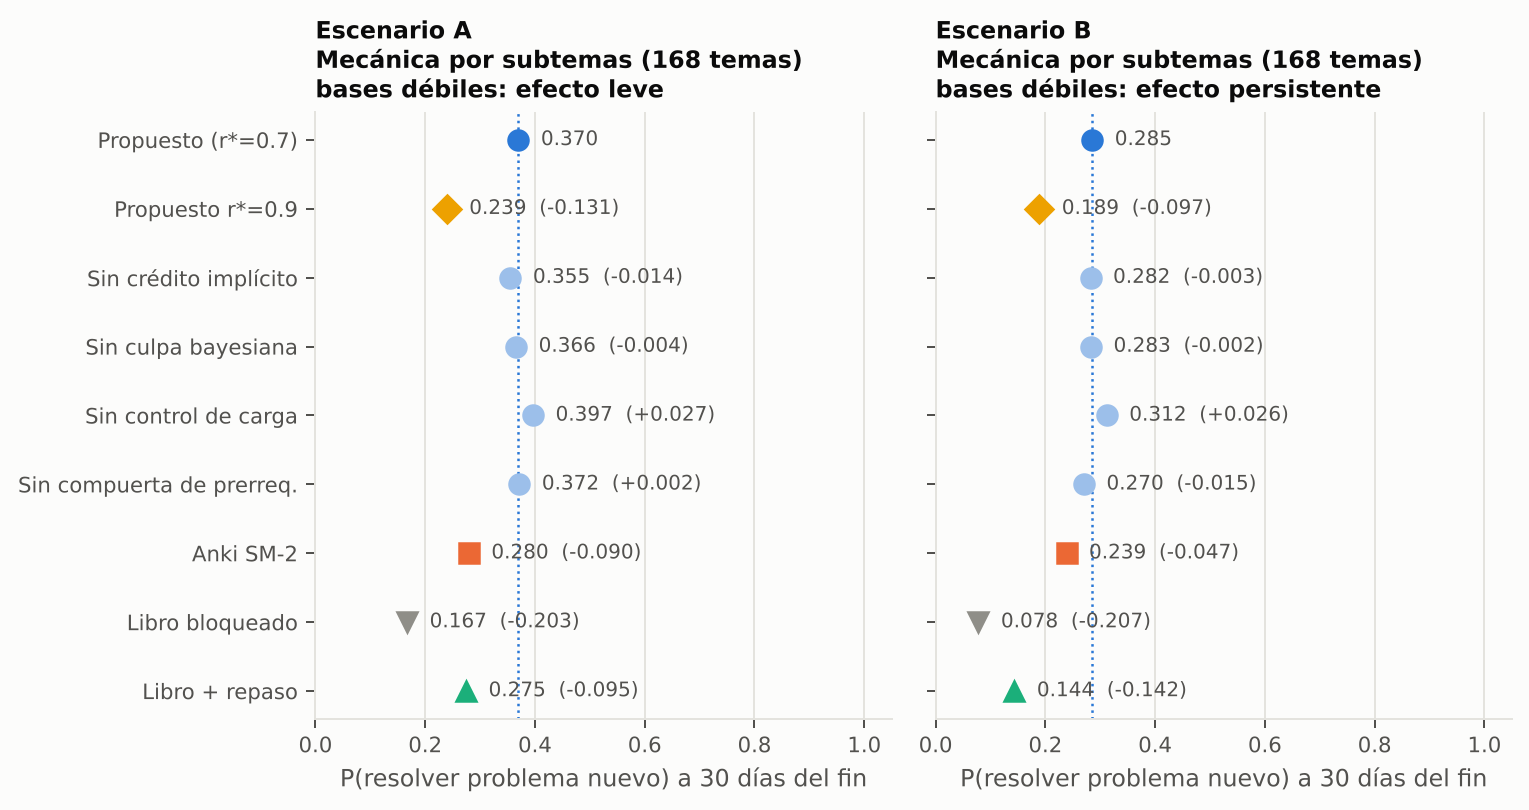
\includegraphics[width=\textwidth]{figuras/subtemas_comparacion.png}
\caption{Grafo de 168 subtemas: examen diferido por política (media $\pm$ IC95\%); entre paréntesis, la diferencia pareada respecto al propuesto. La línea punteada marca el propuesto.}
\label{fig:subtemas}
\vspace{6mm}
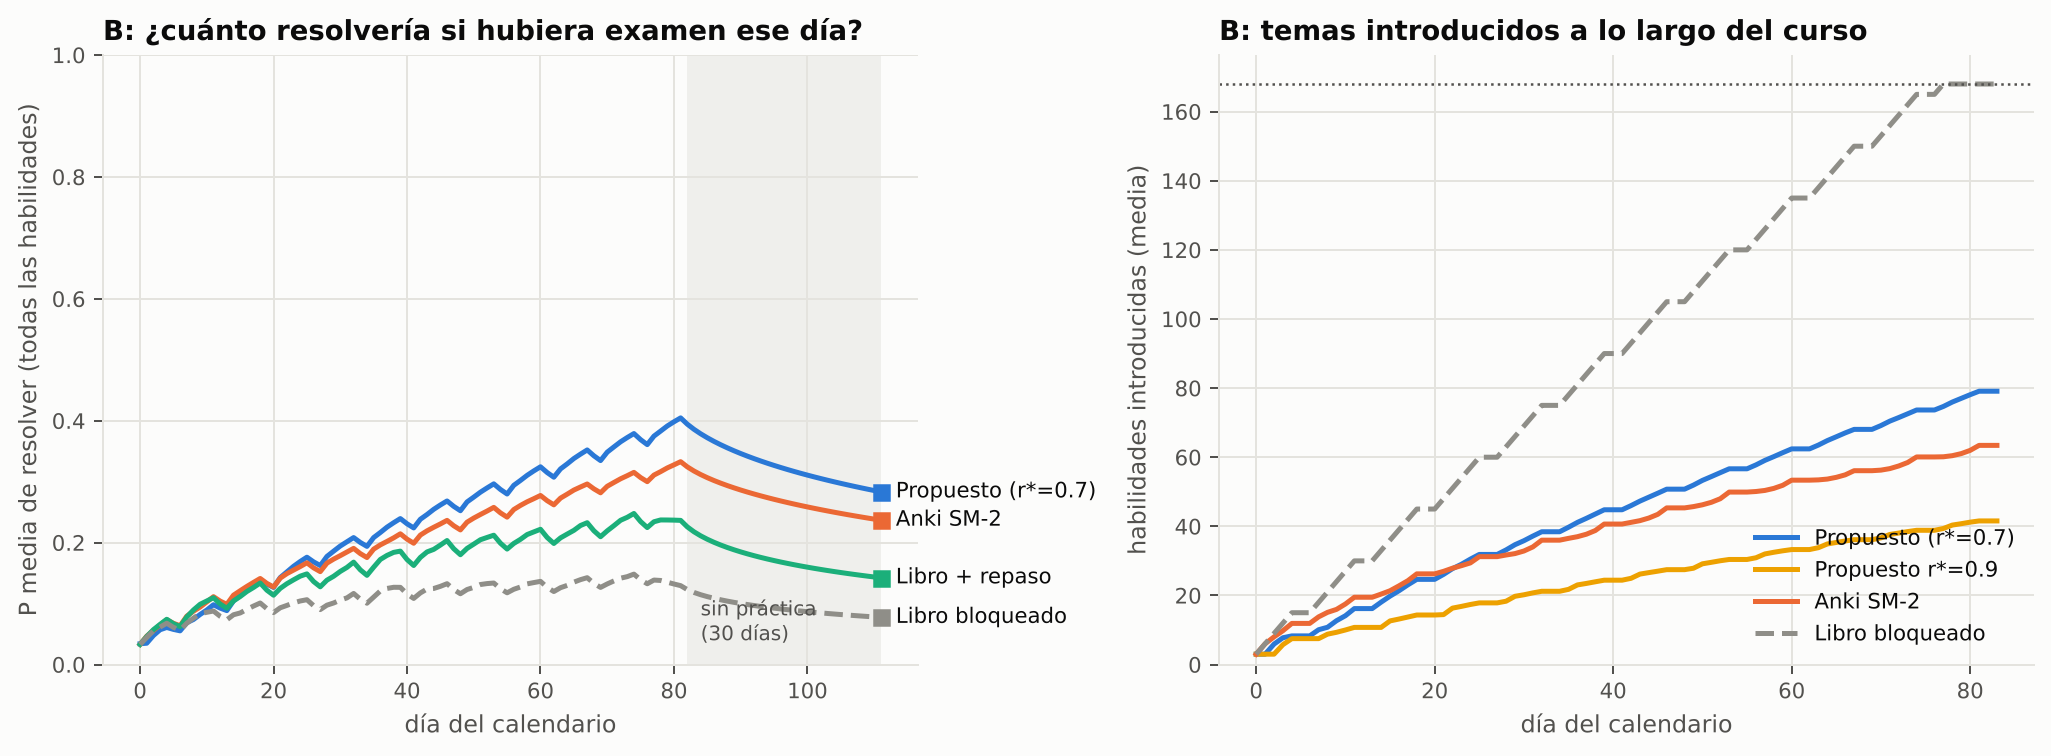
\includegraphics[width=\textwidth]{figuras/subtemas_trayectorias.png}
\caption{Escenario B del grafo de subtemas. Izquierda: probabilidad media de resolver si el examen fuera ese día; la zona gris son los 30 días sin práctica. Derecha: temas introducidos. Anki se atasca con sus repasos vencidos; el propuesto con $\rstar=0.9$ repasa tan seguido que casi no avanza.}
\label{fig:trayectorias}
\end{figure}

\begin{figure}[t]
\centering
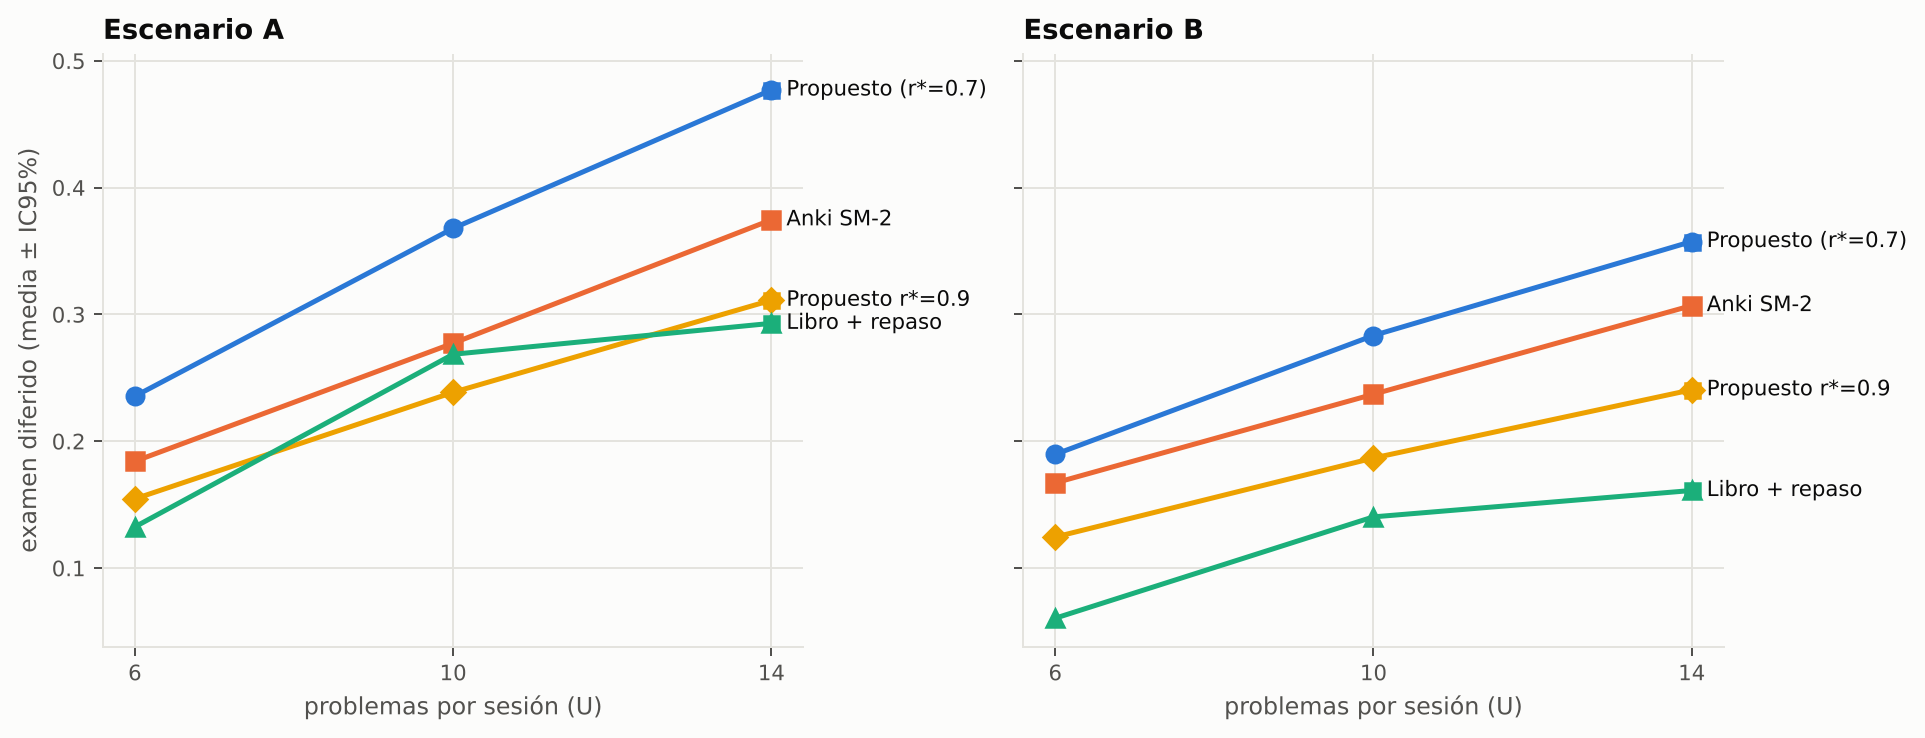
\includegraphics[width=0.92\textwidth]{figuras/subtemas_presupuesto.png}
\caption{Grafo de subtemas: examen diferido según el número de problemas por sesión $U$. La ventaja del propuesto sobre Anki se mantiene en todo el rango.}
\label{fig:presupuesto}
\end{figure}

\paragraph{Cobertura frente a retención.} La métrica~\eqref{eq:examen} mezcla dos cosas. Si se descuenta la contribución $g$ de los temas no introducidos, la probabilidad media \emph{sobre los temas introducidos} es aproximadamente:
\begin{itemize}
\item escenario A: 0.58 con el propuesto, 0.64 con Anki y 0.68 con el propuesto con $\rstar=0.9$;
\item escenario B: 0.58 con el propuesto y 0.60 con Anki.
\end{itemize}
Lo mismo indica la columna $P\ge0.8$: Anki y el propuesto con $\rstar=0.9$ dejan más subtemas ``dominados''. El propuesto con $\rstar=0.7$ gana porque cubre más temas con una retención algo menor por tema. Si el objetivo pedagógico es dominar pocos temas a fondo, la conclusión se invierte. La elección de $\rstar$ es, por lo tanto, una decisión sobre esa frontera y no un detalle técnico.

\subsection{Sensibilidad}

La Figura~\ref{fig:sensibilidad} muestra que bajar $\rstar$ de $0.7$ a $0.5$--$0.6$ mejora todavía más la métrica en el grafo de subtemas ($0.403$ con $\rstar=0.5$ en A), mientras que $\rstar\ge0.9$ la deteriora mucho. El mecanismo es doble: repasar con $\Rh\approx0.9$ rinde poco en la verdad, y la carga estimada~\eqref{eq:carga} se infla y bloquea la admisión. El control de carga resulta conservador: quitarlo mejora la métrica en $+0.027$, al costo de introducir temas con menos retención. En cambio, la compuerta es poco sensible para $\Slisto\le7$ y perjudicial para $\Slisto\ge15$.

\begin{figure}[t]
\centering
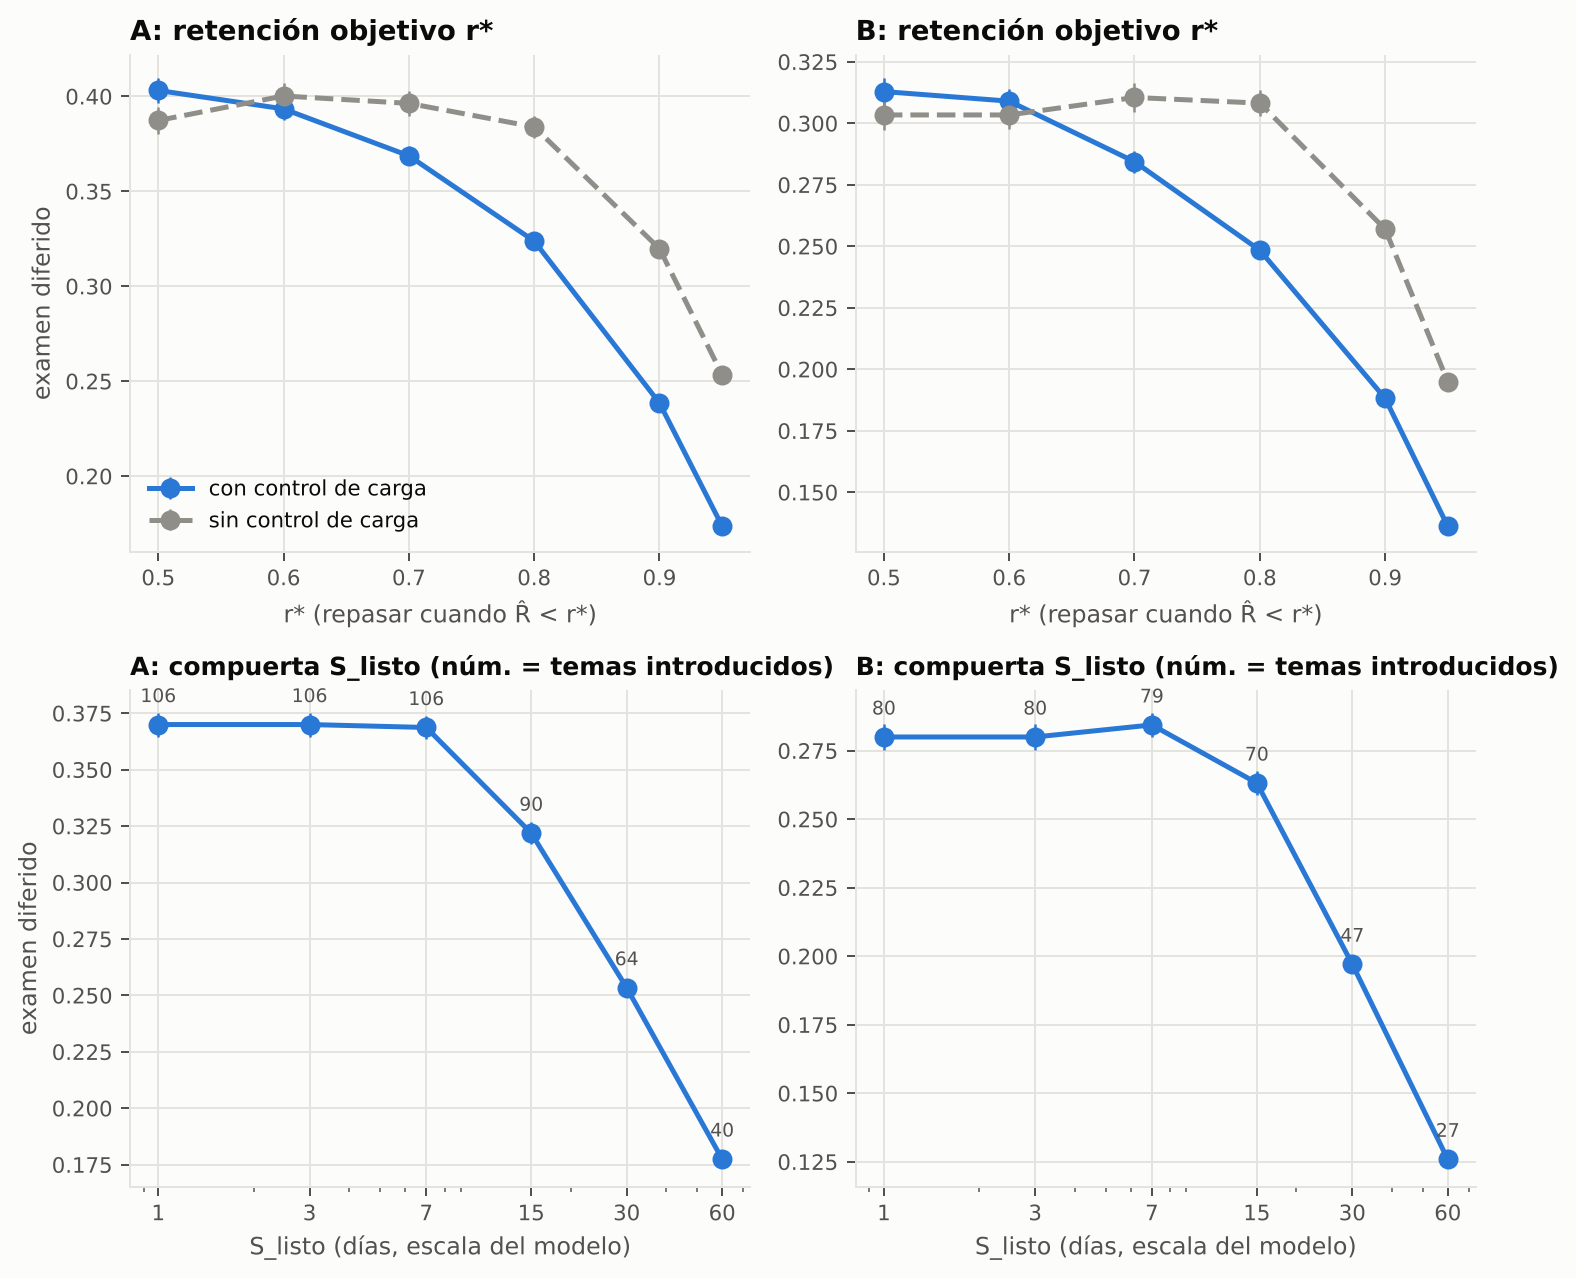
\includegraphics[width=0.85\textwidth]{figuras/subtemas_sensibilidad.png}
\caption{Grafo de subtemas. Arriba: retención objetivo $\rstar$, con y sin control de carga. Abajo: umbral de la compuerta $\Slisto$; los números indican los temas introducidos.}
\label{fig:sensibilidad}
\end{figure}

\subsection{La estructura del grafo importa}

La Tabla~\ref{tab:lineal} compara el grafo de subtemas con dependencias explícitas con la versión de cadenas lineales.
\begin{itemize}
\item En A, la ventaja del propuesto sobre Anki se reduce de $+0.090$ a $+0.012$.
\item En B, el propuesto cae a 0.124 y queda $0.115$ por debajo de Anki. Con 103 niveles de profundidad sólo hay un tema admisible a la vez, y la compuerta deja al sistema con 28 temas en todo el curso. Anki, que ignora el grafo, no sufre.
\end{itemize}
Un grafo con dependencias falsas castiga justamente al sistema que lo respeta: el valor práctico del modelo depende de la fidelidad del grafo tanto como de la regla de repaso. Una advertencia: la normalización de la profundidad ($c_d$) difiere entre ambos grafos (0.30 frente a 0.058), así que la comparación también cambia la dificultad relativa de los temas en la verdad.

\begin{table}[t]
\centering\small
\caption{Dependencias explícitas frente a cadenas lineales (168 subtemas).}
\label{tab:lineal}
\begin{tabular}{lcccc}
\toprule
& \multicolumn{2}{c}{A: efecto leve} & \multicolumn{2}{c}{B: efecto persistente} \\
\cmidrule(lr){2-3}\cmidrule(lr){4-5}
& Dependencias & Lineal & Dependencias & Lineal \\
\midrule
Propuesto & 0.370 & 0.298 & 0.285 & 0.124 \\
Anki SM-2 & 0.280 & 0.286 & 0.239 & 0.238 \\
Propuesto sin compuerta & 0.372 & 0.297 & 0.270 & 0.234 \\
Temas introducidos (propuesto) & 106 & 87 & 79 & 28 \\
\bottomrule
\end{tabular}
\end{table}

\subsection{Calibración del modelo}

Fuera de muestra, sobre los intentos de la política propuesta, el modelo exponencial obtiene AUC de 0.67 y Brier de 0.17--0.18 en el grafo de subtemas, y AUC de 0.66--0.70 en el de unidades (Figura~\ref{fig:calibracion}). Sobreestima la probabilidad de acierto en el rango medio, lo cual es esperable: la verdad usa olvido de ley de potencia y lapsos ocultos. Aun así, el planificador funciona razonablemente bien. La calibración es, por lo tanto, el diagnóstico natural para detectar la mala especificación con datos reales.

\begin{figure}[t]
\centering
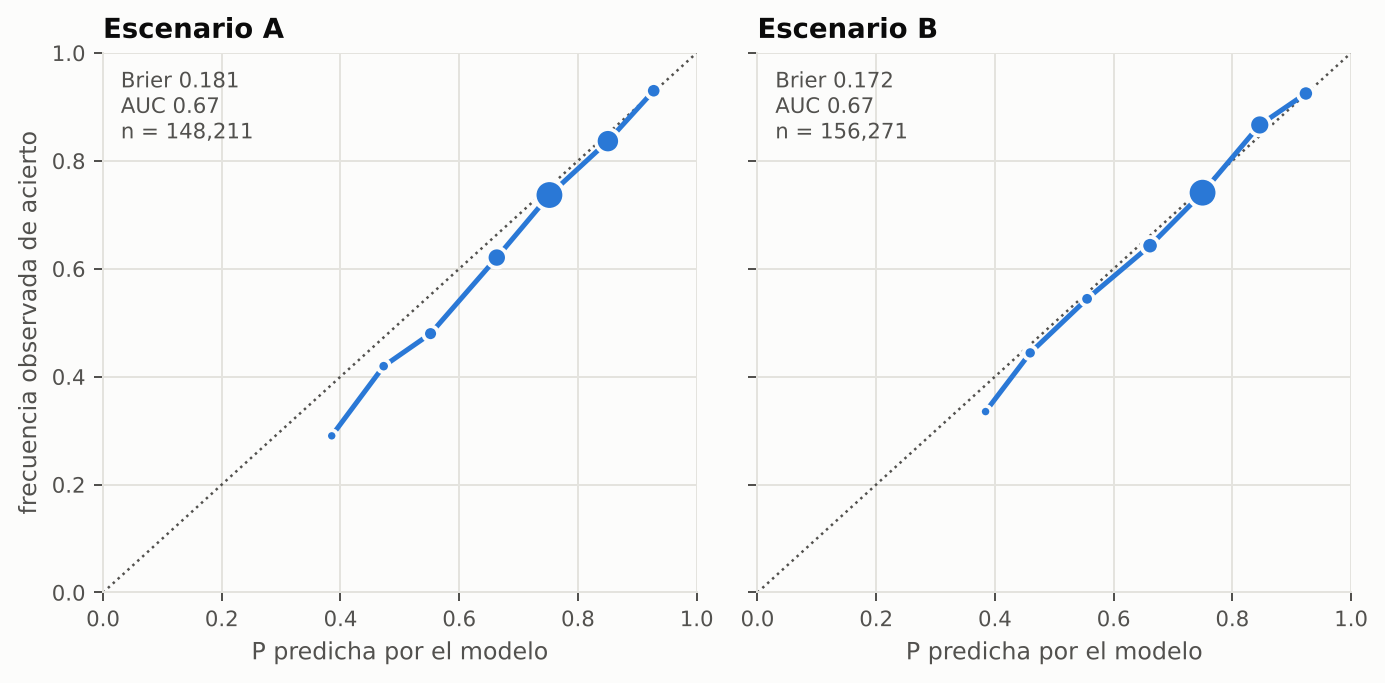
\includegraphics[width=0.75\textwidth]{figuras/subtemas_calibracion.png}
\caption{Calibración fuera de muestra del modelo~\eqref{eq:observacion} en el grafo de subtemas. El tamaño del punto es proporcional al número de intentos del intervalo.}
\label{fig:calibracion}
\end{figure}

%=====================================================================
\section{Discusión y limitaciones}
\label{sec:discusion}
%=====================================================================

\paragraph{Qué importa.} En todos los escenarios, el efecto más grande y robusto es espaciar los repasos frente a la enseñanza bloqueada ($+0.20$ a $+0.29$). Entre políticas espaciadas, la ventaja del modelo propuesto aparece sólo cuando (i) el grafo es de grano fino y el presupuesto es escaso, y (ii) el grafo refleja dependencias reales. Los componentes más finos (culpa bayesiana, crédito implícito, compuerta) tienen efectos pequeños y dependientes del escenario.

\paragraph{Limitaciones.}
\begin{enumerate}
\item \textbf{La verdad es un modelo.} Los resultados indican qué componentes \emph{podrían} importar y bajo qué supuestos, no cuánto se ganará en un aula.
\item \textbf{Elección de $\rstar$ a posteriori.} El valor $\rstar=0.7$ se eligió tras un barrido preliminar. En la tesis debe fijarse con un procedimiento que no use la verdad, por ejemplo optimizándolo en simulación con el modelo ajustado al piloto.
\item \textbf{La métrica favorece la cobertura.} Un $\rstar$ bajo implica más fallos durante la práctica, con posibles costos de motivación que no se modelan.
\item \textbf{Grafo de subtemas.} Las 279 dependencias son un borrador anotado manualmente, pendiente de validación docente. La arista ``tiro parabólico $\to$ aplicaciones de Newton'' del grafo de unidades se omitió por no encontrarse un subtema que la use.
\item \textbf{Simplificaciones del modelo}: $s$ y $g$ fijos, culpa sin $s$ ni $g$~\eqref{eq:culpa}, $\Sh_0$ común a todas las habilidades y sin efectos por alumno. En la variante lineal del escenario B, la estimación $\hat\lambda\approx0$ sugiere problemas de identificabilidad.
\item \textbf{Fenómenos no modelados}: intercalado \citep{rohrer2015}, fatiga, abandono, variación entre instancias de un mismo tipo de problema y aprendizaje por ejemplos resueltos.
\item \textbf{Ruido de examen.} La métrica es la probabilidad esperada, sin el ruido de un examen finito. En un aula, la varianza entre alumnos será mucho mayor.
\end{enumerate}

%=====================================================================
\section{Trabajo futuro y diseño experimental}
\label{sec:futuro}
%=====================================================================

\begin{enumerate}
\item \textbf{Culpa completa}~\eqref{eq:culpa-completa}, y estimación de $s$ y $g$ junto con $\bm\phi$.
\item \textbf{Modelo jerárquico}, $\log\Sh_{0,ik}=\mu_k+\theta_i$, estimado de forma bayesiana (por ejemplo con Stan) con datos del piloto; estimación de los pesos $w_{jk}$ y comparación de las formas exponencial y de potencia por log-verosimilitud predictiva.
\item \textbf{Validación del grafo}: revisión docente de las dependencias y validación empírica de la matriz $Q$ con los datos del piloto.
\item \textbf{Elección de $\rstar$} con un criterio explícito sobre la frontera cobertura--retención.
\item \textbf{Intercalado}: restringir problemas consecutivos del mismo tema principal y evaluarlo como factor.
\item \textbf{Experimento en aula.} Diseño intra-sujeto contrabalanceado al estilo de \citet{lindsey2014}: cada alumno practica dos conjuntos equivalentes de subtemas, uno con cada política (propuesto frente a FSRS o SM-2 con límite de nuevas), con tiempo igualado y una prueba diferida a 30 días con problemas nuevos. Con diferencias pareadas, $n=7.85/d_z^2$ da 32 alumnos para $d_z=0.5$ y 88 para $d_z=0.3$ ($\alpha=0.05$, potencia 0.8). Análisis con modelos mixtos (alumno y subtema como efectos aleatorios) y prerregistro.
\end{enumerate}

%=====================================================================
\appendix
\section{Ejemplo numérico}
\label{app:traza}
%=====================================================================

Seguimos a un alumno promedio ($\theta=0$) en el grafo de la Figura~\ref{fig:grafo-ejemplo}, con $U=3$, $\Sh_0=6.8$, $G=6.18$ y $\lambda=0.19$, durante las sesiones de los días 0--4 y 7--9.

\begin{itemize}
\item \textbf{Día 0.} Se introduce MRU. Los dos problemas de práctica se resuelven con $R=1$, así que no fortalecen la memoria verdadera: $e^{2(1-1)}-1=0$.
\item \textbf{Día 1.} $R_{\text{MRU}}=(1+\tfrac{19}{81}\cdot\tfrac{1}{0.6})^{-0.5}=0.848$ y $\Rh=e^{-1/6.8}=0.863$. MUA no es admisible porque $\Sh_{\text{MRU}}=6.8<\Slisto=7$. Tras un acierto, la verdad pasa de $S=0.60$ a $1.52$ y el modelo de $\Sh=6.80$ a $12.55$.
\item \textbf{Día 2.} MUA se vuelve admisible: $\Sh_{\text{MRU}}=12.55\ge7$ y la carga es $1.4/(12.55\ln(1/0.7))=0.31\le2.4-1$. Al introducirla, la verdad da $S_{\text{MUA}}=0.516\cdot0.931^{0.5}=0.498$, y la práctica de MUA repasa de paso MRU: $\Sh_{\text{MRU}}$ pasa de $12.55$ a $15.52$ y $\Rh$ de $0.923$ a $0.962$.
\item \textbf{Día 7}, tras el fin de semana. Caída libre es la única habilidad vencida ($\Rh=0.643$). La verdad no recupera caída libre ($u=0.935>0.614$) y el problema falla. El modelo reparte la culpa: $b_{\text{caída}}=0.84$, $b_{\text{MUA}}=0.26$, y $\Sh$ pasa de $6.80$ a $5.72$ y de $15.52$ a $14.76$. En la verdad, MUA sí se había recuperado y ganó estabilidad; el modelo no puede saberlo y comete un pequeño error.
\item \textbf{Día 8.} El modelo sobreestima caída libre ($\Rh=0.840$ frente a $R=0.678$), porque el lapso verdadero llevó $S$ al piso. Un problema de MRU falla por descuido ($u=0.043<s$) sin dañar la memoria.
\end{itemize}

%=====================================================================
\begin{thebibliography}{99}
\small

\bibitem[{Arthur et~al.(1998)}]{arthur1998}
Arthur, W., Bennett, W., Stanush, P.~L. y McNelly, T.~L. (1998).
\newblock Factors that influence skill decay and retention: A quantitative review and analysis.
\newblock \emph{Human Performance}, 11(1):57--101.

\bibitem[{Barzagar~Nazari y Ebersbach(2019)}]{barzagar2019}
Barzagar~Nazari, K. y Ebersbach, M. (2019).
\newblock Distributing mathematical practice of third and seventh graders: Applicability of the spacing effect in the classroom.
\newblock \emph{Applied Cognitive Psychology}, 33(2):288--298.

\bibitem[{Cen et~al.(2006)}]{cen2006}
Cen, H., Koedinger, K. y Junker, B. (2006).
\newblock Learning factors analysis: A general method for cognitive model evaluation and improvement.
\newblock En \emph{Intelligent Tutoring Systems (ITS 2006)}, pp.~164--175. Springer.

\bibitem[{Cepeda et~al.(2006)}]{cepeda2006}
Cepeda, N.~J., Pashler, H., Vul, E., Wixted, J.~T. y Rohrer, D. (2006).
\newblock Distributed practice in verbal recall tasks: A review and quantitative synthesis.
\newblock \emph{Psychological Bulletin}, 132(3):354--380.

\bibitem[{Cepeda et~al.(2008)}]{cepeda2008}
Cepeda, N.~J., Vul, E., Rohrer, D., Wixted, J.~T. y Pashler, H. (2008).
\newblock Spacing effects in learning: A temporal ridgeline of optimal retention.
\newblock \emph{Psychological Science}, 19(11):1095--1102.

\bibitem[{Choffin et~al.(2019)}]{choffin2019}
Choffin, B., Popineau, F., Bourda, Y. y Vie, J.-J. (2019).
\newblock DAS3H: Modeling student learning and forgetting for optimally scheduling distributed practice of skills.
\newblock En \emph{Proceedings of the 12th International Conference on Educational Data Mining (EDM 2019)}. arXiv:1905.06873.

\bibitem[{Choffin et~al.(2021)}]{choffin2021}
Choffin, B., Popineau, F. y Bourda, Y. (2021).
\newblock Extending adaptive spacing heuristics to multi-skill items.
\newblock \emph{Journal of Educational Data Mining}, 13(3).

\bibitem[{Corbett y Anderson(1994)}]{corbett1994}
Corbett, A.~T. y Anderson, J.~R. (1994).
\newblock Knowledge tracing: Modeling the acquisition of procedural knowledge.
\newblock \emph{User Modeling and User-Adapted Interaction}, 4(4):253--278.

\bibitem[{de~la Torre(2011)}]{delatorre2011}
de~la Torre, J. (2011).
\newblock The generalized DINA model framework.
\newblock \emph{Psychometrika}, 76(2):179--199.

\bibitem[{Doignon y Falmagne(1985)}]{doignon1985}
Doignon, J.-P. y Falmagne, J.-C. (1985).
\newblock Spaces for the assessment of knowledge.
\newblock \emph{International Journal of Man-Machine Studies}, 23(2):175--196.

\bibitem[{Hunziker et~al.(2019)}]{hunziker2019}
Hunziker, A., Chen, Y., Mac~Aodha, O., Gomez-Rodriguez, M., Krause, A., Perona, P., Yue, Y. y Singla, A. (2019).
\newblock Teaching multiple concepts to a forgetful learner.
\newblock En \emph{Advances in Neural Information Processing Systems 32 (NeurIPS 2019)}.

\bibitem[{Junker y Sijtsma(2001)}]{junker2001}
Junker, B.~W. y Sijtsma, K. (2001).
\newblock Cognitive assessment models with few assumptions, and connections with nonparametric item response theory.
\newblock \emph{Applied Psychological Measurement}, 25(3):258--272.

\bibitem[{Koedinger et~al.(2012)}]{koedinger2012}
Koedinger, K.~R., Corbett, A.~T. y Perfetti, C. (2012).
\newblock The Knowledge-Learning-Instruction framework: Bridging the science-practice chasm to enhance robust student learning.
\newblock \emph{Cognitive Science}, 36(5):757--798.

\bibitem[{Lindsey et~al.(2014)}]{lindsey2014}
Lindsey, R.~V., Shroyer, J.~D., Pashler, H. y Mozer, M.~C. (2014).
\newblock Improving students' long-term knowledge retention through personalized review.
\newblock \emph{Psychological Science}, 25(3):639--647.

\bibitem[{Nemhauser et~al.(1978)}]{nemhauser1978}
Nemhauser, G.~L., Wolsey, L.~A. y Fisher, M.~L. (1978).
\newblock An analysis of approximations for maximizing submodular set functions---I.
\newblock \emph{Mathematical Programming}, 14(1):265--294.

\bibitem[{Pavlik et~al.(2009)}]{pavlik2009}
Pavlik, P.~I., Cen, H. y Koedinger, K.~R. (2009).
\newblock Performance factors analysis: A new alternative to knowledge tracing.
\newblock En \emph{Artificial Intelligence in Education (AIED 2009)}, pp.~531--538. IOS Press.

\bibitem[{Pyc y Rawson(2009)}]{pyc2009}
Pyc, M.~A. y Rawson, K.~A. (2009).
\newblock Testing the retrieval effort hypothesis: Does greater difficulty correctly recalling information lead to higher levels of memory?
\newblock \emph{Journal of Memory and Language}, 60(4):437--447.

\bibitem[{Reddy et~al.(2016)}]{reddy2016}
Reddy, S., Labutov, I., Banerjee, S. y Joachims, T. (2016).
\newblock Unbounded human learning: Optimal scheduling for spaced repetition.
\newblock En \emph{Proceedings of the 22nd ACM SIGKDD International Conference on Knowledge Discovery and Data Mining}, pp.~1815--1824.

\bibitem[{Rohrer et~al.(2015)}]{rohrer2015}
Rohrer, D., Dedrick, R.~F. y Stershic, S. (2015).
\newblock Interleaved practice improves mathematics learning.
\newblock \emph{Journal of Educational Psychology}, 107(3):900--908.

\bibitem[{Rohrer y Taylor(2007)}]{rohrer2007}
Rohrer, D. y Taylor, K. (2007).
\newblock The shuffling of mathematics problems improves learning.
\newblock \emph{Instructional Science}, 35(6):481--498.

\bibitem[{Skycak(2023)}]{skycak2023}
Skycak, J. (2023).
\newblock Individualized spaced repetition in hierarchical knowledge structures.
\newblock \url{https://www.justinmath.com/individualized-spaced-repetition-in-hierarchical-knowledge-structures/}.

\bibitem[{Su et~al.(2023)}]{su2023}
Su, J., Ye, J., Nie, L., Cao, Y. y Chen, Y. (2023).
\newblock Optimizing spaced repetition schedule by capturing the dynamics of memory.
\newblock \emph{IEEE Transactions on Knowledge and Data Engineering}, 35(10):10085--10097.

\bibitem[{Tabibian et~al.(2019)}]{tabibian2019}
Tabibian, B., Upadhyay, U., De, A., Zarezade, A., Schölkopf, B. y Gomez-Rodriguez, M. (2019).
\newblock Enhancing human learning via spaced repetition optimization.
\newblock \emph{Proceedings of the National Academy of Sciences}, 116(10):3988--3993.

\bibitem[{Tatsuoka(1983)}]{tatsuoka1983}
Tatsuoka, K.~K. (1983).
\newblock Rule space: An approach for dealing with misconceptions based on item response theory.
\newblock \emph{Journal of Educational Measurement}, 20(4):345--354.

\bibitem[{Upadhyay et~al.(2021)}]{upadhyay2021}
Upadhyay, U., Lancashire, G., Moser, C. y Gomez-Rodriguez, M. (2021).
\newblock Large-scale randomized experiments reveals that machine learning-based instruction helps people memorize more effectively.
\newblock \emph{npj Science of Learning}, 6:26.

\bibitem[{Woźniak(1990)}]{wozniak1990}
Woźniak, P.~A. (1990).
\newblock \emph{Optimization of learning}.
\newblock Tesis de maestría, Universidad Tecnológica de Poznań.

\bibitem[{Ye et~al.(2022)}]{ye2022}
Ye, J., Su, J. y Cao, Y. (2022).
\newblock A stochastic shortest path algorithm for optimizing spaced repetition scheduling.
\newblock En \emph{Proceedings of the 28th ACM SIGKDD Conference on Knowledge Discovery and Data Mining}, pp.~4381--4390.

\end{thebibliography}

\end{document}
